\documentclass[12pt,a4paper]{article}
\usepackage[utf8]{inputenc}
\usepackage[margin=2cm]{geometry}
\usepackage{amsmath}
\usepackage{amssymb}
\usepackage{amsthm} 
\usepackage{graphicx}
\usepackage{mathtools}
\usepackage{ textcomp }
\usepackage{amsthm}
\usepackage[normalem]{ulem}
\DeclarePairedDelimiter{\abs}{\lvert}{\rvert}
\DeclarePairedDelimiter{\norma}{\lVert}{\rVert}
\DeclarePairedDelimiter{\normaA}{\big | |}{|  \big |}
\newcommand{\inter}{\begin{matrix}\prod\end{matrix}}
 
\begin{document}

\section{Lezione 19 - Norme vettoriali e matriciali}
%PAGINA 1\\%mike
Con questa lezione entriamo nel mondo dell'Algebra Lineare Numerica (NLA in inglese, Numerical Linear Algebra), cioè quel vastissimo capitolo del calcolo numerico che ha a che fare con la soluzione approssimata al calcolatore di sistemi lineari, il calcolo di fattorizzazioni di matrici
%PAGINA 2\\%mike
e funzioni di matrici, il calcolo di trasformate lineari, di autovalori e autovettori,..\\Come si scopre aprendo un qualsiasi testo esteso di calcolo numerico, l'algebra lineare numerica occupa una parte molto consistente della materia.\\In effetti i metodi dell'algebra lineare numerica sono pervasivi e di importanza fondamentale nei più svariati ambiti applicativi, dalla modellistica numerica con equazioni differenziali all'elaborazione di
%PAGINA 3\\%mike
segnali e immagini, alla ``data science",..\\Il motivo è che non solo ci sono moltissimi modelli lineari discreti o discretizzati che portano direttamente ad un problema di algebra lineare, ma che anche nel trattamento di problemi e modelli non lineari un approccio tipico è una qualche forma di \uline{linearizzazione}, spesso iterativa.\\Si pensi ad esempio quel metodo di Newton, un classico esempio di linearizzazione iterativa di un problema non lineare; bene,
%PAGINA 4\\%mike
noi lo abbiamo visto per singole equazioni, ma il metodo si può estendere a \uline{sistemi} di equazioni non lineari, grazie agli strumenti del calcolo differenziale in più variabili, risolvendo un sistema lineare tramite una successione di sistemi lineari, le cui soluzioni (che sono vettori) convergono alla soluzione (che è un vettore) del sistema lineare.\\L'algebra lineare numerica è un mondo di \uline{vettori e matrici}
%PAGINA 5\\%mike
(le quali rappresentano  le trasformazioni lineari che agiscono sui vettori) in cui tutte le quantità con cui si opera (gli elementi dei vettori e delle matrici) non sono in pratica mai esatte ma affette da errori (di arrotondamento, di misura nel caso di dati sperimentali, di propagazione,..).\\Diventa quindi essenziale avere dei modi per misurare gli errori su vettori e matrici, come strumento di base nell'analisi degli algoritmi numerici per la
%PAGINA 6\\%mike
soluzione approssimata dei problemi dell'algebra lineare.\\
Anticipiamo che in questo corso ci occuperemo solo della soluzione di sistemi lineari
\begin{equation*}
    Ax=b,\quad A\in\mathbb{R}^{m\times n}, \quad x\in\mathbb{R}^n,\quad b\in\mathbb{R}^m
\end{equation*}
per $m=n$ (sistemi determinati) e $m>n$ (sistemi sovradeterminati) utilizzando due tra i principali metodi ``diretti", cioè metodi che arrivano alla soluzione tramite un numero finito di passi di trasformazione di $A$ e $b$, ovvero il \uline{\textbf{METODO DI ELIMINAZIONE di GAUSS}} per sistemi determinati
%PAGINA 7\\%mike
non singolari ($A$ invertibile) e il \uline{\textbf{METODO DEI MINIMI QUADRATI}} per sistemi sovradeterminati.\\In entrambi i casi un aspetto chiave sarà legato a una speciale \uline{fattorizzazione} della matrice del sistema nel prodotto di due matrici con particolare struttura (la fattorizzazione LU prodotto di due matrici triangolari e la fattorizzazione QR prodotto di una matrice ortogonale per una matrice triangolare).\\Questi metodi diretti sono metodi
%PAGINA 8\\%mike
``general purpose", nel senso che sono applicabili a sistemi generali senza bisogno di sfruttare particolari proprietà delle matrici.\\Non ci occuperemo dei cosiddetti ``metodi iterativi", l'altra grande famiglia di algoritmi per la soluzione numerica di sistemi lineari, che sono specializzati su classi di matrici con particolari proprietà e costruiscono in vari modi \uline{successioni} di vettori che convergono al vettore soluzione del sistema.\\Pur non occupandocene, nel
%PAGINA 9 \\ % michele
resto di questa lezione daremo gli strumenti concettuali per misurare vettori e matrici e gli errori su questi oggetti, strumenti che permettono fra l'altro di definire il concetto di convergenza in ambito vettoriale. Iniziamo parlando di

\subsection{Norme vettoriali}
Nel seguito ci occuperemo di vettori $n$-dimensionali reali, $x = (x_1, \dotso, x_n) \in \mathbb{R}^n$, anche se molte delle definizioni e delle proprietà si possono estendere
%PAGINA 10-11 \\ % michele
a vettori complessi $(x \in \mathbb{C}^n)$ con le opportune varianti quando necessario (ad esempio il prodotto scalare $(x,y) = \sum\limits_{i=1}^n x_i \cdot y_i$ diventa per vettori complessi $(x,y) = \sum\limits_{i=1}^n x_i \cdot \overline{y_i}$, dove $\overline{y_i}$ è il coniugato).

\subsubsection{Definizione}
Una NORMA vettoriale in $\mathbb{R}^n$ è una funzione
\[
\norma{\cdot} : \mathbb{R}^n \to [ 0, + \infty ), \quad x \mapsto \norma{x}
\]
con le seguenti proprietà:
\begin{enumerate}
    \item $\norma{x+y} \le \norma{x} + \norma{y}, \quad \forall x,y \in \mathbb{R}^n$ [per la disuguaglianza triangolare]
    
    \item $\norma{\alpha x} = \abs{\alpha} \norma{x}, \quad \forall \alpha \in \mathbb{R}, \quad \forall x \in \mathbb{R}^n$
    
    \item $\norma{x} = 0 \iff x = 0 = (0, \dotso , 0)$ [vettore nullo]
\end{enumerate}
Si dimostra facilmente che vale
\[
\norma{x+y} \ge \abs{\norma{x} - \norma{y}} \quad \forall x, y \in \mathbb{R}^n
\]
Quindi la disuguaglianza triangolare è una generalizzazione del caso $n=1$ con $\norma{x} = \abs{x}, \ x \in \mathbb{R}$, per cui vale come sappiamo
\[
\abs{\abs{x} - \abs{y}} \le \abs{x+y} \le \abs{x} + \abs{y}
\]

\subsubsection{Norma euclidea}
Una norma è in un certo senso una ``lunghezza" del vettore.\\
In effetti una delle norme più usate è la norma ``euclidea" detta anche \textit{norma-2}
%PAGINA 12 \\ % michele
\[
\norma{x}_2 = \sqrt{\sum_{i=1}^n x_i^2} = \sqrt{(x,x)}
\]
che per $n=2$ e $n=3$ rappresenta geometricamente proprio la lunghezza del vettore $x$ (via teorema di Pitagora).\\

\subsubsection{Norma-infinito}
Altre due norme molto usate sono la norma del massimo modulo detta \textit{norma-infinito}
\[
\norma{x}_\infty = \underset{1 \le i \le n}{\text{max}} \ \abs{x_i}
\]

\subsubsection{Norma-1}
e la \textit{norma-1}
\[
\norma{x}_1 = \sum_{i=1}^n \abs{x_i}
\]
%PAGINA 13 \\ % michele

\subsubsection{Norma-p}
Più in generale la \textit{norma-p} è
\[
\norma{x}_p = \left(\sum_{i=1}^n \abs{x_i}^p\right)^{1/p}, \quad p \ge 1
\]

\subsubsection{Distanza tra vettori}
Una volta scelta una norma (esistono infinite norme) possiamo definire una distanza tra vettori nel modo seguente
\[
dist_{\norma{\cdot}} (x,y) = \norma{x-y}
\]
e quindi possiamo misurare quando un vettore è vicino a un altro vettore, cioè possiamo misurare l'errore su un vettore.\\
In particolare, possiamo definire un intorno (chiuso) di raggio $\varepsilon$ di $x \in \mathbb{R}^n$ nel modo seguente
%PAGINA 14 \\%Alessandro
\begin{equation*}
    I_\varepsilon(x)=\left\{ y \in \mathbb{R}^n : \norma{x-y} \leq \varepsilon \right\}
\end{equation*}
cioè l'insieme degli infiniti vettori che distano non più di $\varepsilon$ da $x$ (detto centro dell'intorno). \\
Un intorno aperto è definito tramite la diseguaglianza stretta 
\begin{equation*}
    \Dot{I}_\varepsilon (x) = \left\{ y \in \mathbb{R}^n : \norma{x-y}<\varepsilon \right\}
\end{equation*}
La forma geometrica degli intorni dipende dalla norma, come si vede in questo disegno per $n=2$
\begin{center}
    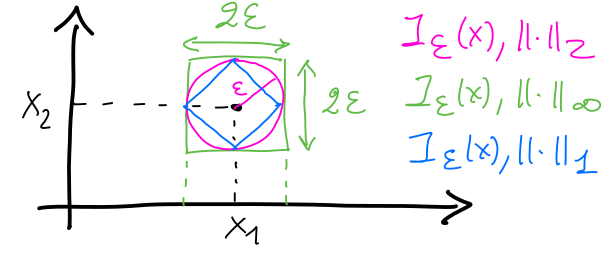
\includegraphics[scale=0.5]{pag14.png}    
\end{center}
%PAGINA 15 \\ %Alessandro
cioè un intorno di raggio $\varepsilon$ in $\norma{\cdot}_2$ è un cerchio di raggio $\varepsilon$ (una sfera piena in $\mathbb{R}^3$, una ipersfera piena in $\mathbb{R}^n$), in $\norma{\cdot}_\infty$ è un quadrato di lato $2\varepsilon$ (un cubo in $\mathbb{R}^3$ e un ipercubo in $\mathbb{R}^n$), in $\norma{\cdot}_1$ è un quadrato con le diagonali parallele agli assi coordinati cioè un quadrato ruotato di $45^\circ$ (la cosa si complica in dimensione $>2$, ad es. in $\mathbb{R}^3$ è un ottaedro regolare con diagonali interne parallele agli assi coord.). \\
Si noti che $I_\varepsilon(x) = I_\varepsilon(0) + x = \left\{ y \in \mathbb{R}^n : y = x+z, \ z \in I_\varepsilon(0) \right\}$,
%PAGINA 16 \\%Alessandro
cioè gli intorni di $x \in \mathbb{R}^n$ sono intorni di 0 traslati per centrarli di $x$.

\subsubsection{Equivalenza tra norme in $\mathbb{R}^n$}
Una proprietà importante è che due norme qualsiasi in $\mathbb{R}^n$ sono ``equivalenti", nel senso che date $\norma{\cdot}_A$ e $\norma{\cdot}_B$ $\exists c_1, c_2 > 0$ tali che  $c_2\norma{x}_B \leq \norma{x}_A \leq c_1\norma{x}_B$. \\
Ad esempio, siccome 
\begin{equation*}
        \norma{x}_2^2 = \sum_{i=1}^n x_i^2 \leq \sum_{i=1}^n (max\lvert x_i \rvert)^2 = \norma{x}_\infty^2 \sum_{i=1}^n 1 = n \norma{x}_\infty^2
\end{equation*}
e
\begin{equation*}
    \norma{x}_\infty^2 = \underset{i}{max}\lvert x_i \rvert^2 \leq \sum_{i=1}^n x_i^2
\end{equation*}
si ha che 
\begin{equation*}
    \underset{=c_2}{1} \cdot \norma{x}_\infty \leq \norma{x}_2 \leq \underset{=c_1}{\sqrt{n}} \norma{x}_\infty
\end{equation*}
%PAGINA 17 \\ %Alessandro
Avendo delle distanze possiamo dire quando una successione $\left\{ x^{(k)} \right\}$ di vettori di $\mathbb{R}^n$ converge a $x \in \mathbb{R}^n$, cioè $dist_{\norma{\cdot}}(x,x^{(k)}) = \norma{x-x^{(k)}} \rightarrow 0, \ k \rightarrow \infty$.\\
Vista l'equivalenza tra coppie di norme, questa nozione di convergenza (e quindi la nozione di limite) \uline{non} dipende dalla norma.\\
Infatti se $\norma{x-x^{(k)}}_A \rightarrow 0$ allora $\norma{x-x^{(k)}}_B \leq \frac{1}{c_2}\norma{x-x^{(k)}}_A \rightarrow 0$ e analogamente se $\norma{x-x^{(k)}}_B \rightarrow 0$ allora $\norma{x-x^{(k)}}_A \leq c_1 \norma{x-x^{(k)}}_B \rightarrow 0$. \\
Si vede subito che $lim_{k\to \infty} x^{(k)} = x$
%PAGINA 18 \\ %Alessandro
se e solo se $(x^{(k)})_i \rightarrow x_i, \ k \to \infty$ (cioè se le componenti $i$-esime convergono $\forall i$ alla componente $i$-esima del vettore limite): basta infatti considerare $\norma{x-x_k}_\infty$ (che è equivalente nel senso detto a tutte le altre norme).\\
Per concludere, possiamo dire che con una norma siamo in grado di ``misurare" i vettori, le distanze tra vettori e gli errori sui vettori.

\subsubsection{Norma matriciale}
Passiamo ora alla nozione di NORMA MATRICIALE.\\
%PAGINA 19 \\%Alessandro
Per semplicità ci restringiamo al caso di matrici quadrate
\begin{equation*}
    A\in \mathbb{R}^{n\times n}=\begin{pmatrix}
 a_{11} & \dots  & a_{1n}\\ 
 a_{21} & \dots  & a_{2n}\\ 
 \vdots &  & \vdots\\ 
 a_{n1} & \dots  & a_{nn} 
\end{pmatrix}
\end{equation*}
Se vediamo semplicemente una matrice come una tabella $n \times n$, cioè un vettore di $\mathbb{R}^{n \times n}$ con $n^2$ elementi organizzato in tabella, una norma di matrice è una qualsiasi norma in $\mathbb{R}^{n^2}$. \\
Ma questo non è il modo giusto di considerare una matrice in algebra lineare.\\
%PAGINA 20\\
Infatti in algebra lineare una matrice rappresenta un operatore lineare che trasforma vettori (visti come vettori colonna) in vettori con la regola
\begin{equation*}
    Ax=A\begin{pmatrix}
        x_1\\
        \vdots\\
        x_n
    \end{pmatrix}
    =\left(\sum_{j=1}^na_{ij}x_j\right)_{1\leq i\leq n}
\end{equation*}
La trasformazione è lineare perchè $\forall\alpha,\beta\in\mathbb{R}$ e $x,y\in\mathbb{R}^n$
\begin{equation*}
    A(\alpha x+\beta y)=\alpha Ax+\beta Ay
\end{equation*}

\subsection{Norma indotta}
Vedendo una matrice nel suo ruolo di trasformazione lineare, fissata una norma vettoriale $\norma{\cdot}$
%PAGINA 21\\
in $\mathbb{R}^n$ possiamo definire una norma in $\mathbb{R}^{n\times n}$ nel modo seguente 
\begin{equation*}
    \norma{A}=\underset{x\neq0}{sup}\frac{\norma{Ax}}{\norma{x}}
\end{equation*}
Si può dimostrare (non richiesto) che tale $sup$ è finito e che vale
\begin{equation*}
    \norma{A}=\underset{x\neq0}{sup}\frac{\norma{Ax}}{\norma{x}}=\underset{\norma{z}=1}{sup}\norma{Az}
\end{equation*}
Una norma matriciale di questo tipo si dice \uline{NORMA INDOTTA} della norma vettoriale $\norma{\cdot}$.
Possiamo verificare facilmente che soddisfa le 3 proprietà
%PAGINA 22 - 23\\ % michele
caratteristiche delle norme
\begin{itemize}
    \item la disuguaglianza triangolare viene da
    \[
    \norma{(A_1 + A_2)x} = \norma{A_1x + A_2x} \le \norma{A_1x} + \norma{A_2x}
    \]
    quindi
\begin{align*}
        \underset{x \neq 0}{sup} \frac{\norma{(A_1 + A_2)x}}{\norma{x}} & \le \underset{x \neq 0}{sup} \frac{\norma{A_1x} + \norma{A_2x}}{\norma{x}} \\
        & \le \underset{x \neq 0}{sup} \frac{\norma{A_1x}}{\norma{x}} + \underset{x \neq 0}{sup} \frac{\norma{A_2x}}{\norma{x}} \\
        & = \norma{A_1} + \norma{A_2}
    \end{align*}
    
    \item per $\alpha \in \mathbb{R}$
    \[
    \norma{\alpha A} = \underset{x \neq 0}{sup} \frac{\norma{\alpha Ax}}{\norma{x}}
    = \underset{x \neq 0}{sup} \frac{\abs{\alpha} \norma{Ax}}{\norma{x}} = \abs{x} \norma{A}
    \]
    
    \item se $\norma{A} = 0$ allora \[\underset{x \neq 0}{sup} \frac{\norma{Ax}}{\norma{x}} = 0\]
    quindi $\norma{Ax} = 0 \quad \forall x \Rightarrow A = 0$ [matrice nulla]
\end{itemize}
Prima di fare esempi di norme matriciali indotte, mostriamo che per esse valgono due

\subsubsection{Disuguaglianze fondamentali per le norme matriciali indotte}
\begin{enumerate}
    \item[i.] $\norma{Ax} \le \norma{A} \cdot \norma{x} \quad \forall A \in \mathbb{R}^{n \times n} \quad \forall x \in \mathbb{R}^n$
    
    \item[ii.] $\norma{AB} \le \norma{A} \cdot \norma{B} \quad \forall A, B \in \mathbb{R}^{n \times n}$
\end{enumerate}


\begin{proof}[\unskip\nopunct]
\uline{Dimostrazione}
\begin{enumerate}
\item[i.] Per quando riguarda (i) basta ricordare la definizione di norma
%PAGINA 24\\
indotta, se $\underset{x \neq 0}{sup} \frac{\norma{Ax}}{\norma{x}} = \norma{A}$ allora 
\[\forall \, x \quad \frac{\norma{Ax}}{\norma{x}} \le sup = \norma{A}\]

\item[ii.] Invece (ii) viene dal significato del prodotto $AB$ come composizione (trasformazione lineare COMPOSTA) delle due trasf. lineari $A$ e $B$
\[ABx = A(Bx)\]
Quindi
\[\norma{ABx} = \norma{A(Bx)} \underbrace{\le \norma{A} \cdot \norma{Bx} \le \norma{A} \cdot \norma{B} \cdot \norma{x}}_{\text{per la (1)}}\]
da cui $\forall x \ne 0$
\[\frac{\norma{ABx}}{\norma{x}} \le \norma{A} \norma{B}\]
e perciò
\[\norma{AB} = \underset{x \neq 0}{sup} \frac{\norma{ABx}}{\norma{x}} \le \norma{A} \norma{B}\]
\end{enumerate}
\end{proof}
%PAGINA 25\\
La (ii) si può parafrasare dicendo che una qualsiasi norma matriciale indotta ``rispetta il prodotto" (ricordiamo per inciso che il prodotto tra matrici non gode della proprietà commutativa).\\ Ciò non è vero per qualsiasi norma in $\mathbb{R}^{n\times n}$: ci sono norme (non indotte) per cui $\exists A,B$ tali che $\norma{AB}>\norma{A}\cdot\norma{B}$. Un esempio è la norma
\begin{equation*}
    \norma{A}=\underset{i,j}{max}|a_{ij}|
\end{equation*}
(si verifica facilmente che ha le 3 proprietà caratteristiche di una
%PAGINA 26 \\%silvia
norma). \\
Possiamo fare un semplice esempio con $n = 2$
\[A = B = \begin{pmatrix}
    1 & 1 \\
    0 & 1
\end{pmatrix}, \quad AB = A^2 =
\begin{pmatrix}
    1 & 2 \\
    0 & 1
\end{pmatrix}\]
Abbiamo $\norma{A} = 1$ e $\norma{A^2} = 2 > \norma{A}^2 = 1$.\\
Quindi 
\[\norma{A} = \max_{i,j} \abs{a_{ij}}\]
non rispetta la moltiplicazione (e di conseguenza \uline{non} può essere indotta da alcuna norma vettoriale).

\subsubsection{Norme indotte notevoli}
Mostriamo ora chi sono le norme matriciali indotte da
%PAGINA 27-28 \\%silvia
$\norma{\cdot}_{\infty}$, $\norma{\cdot}_2$ e $\norma{\cdot}_1$ in $\mathbb{R}^n$.\\
\begin{itemize}
    \item La prima, che viene chiamata $\norma{A}_{\infty}$ è
    \[\norma{A}_{\infty} = \sup_{x \ne 0} \frac{\norma{Ax}_{\infty}}{\norma{x}_{\infty}} = \max_{1 \le i \le n} \sum_{j=1}^n \abs{a_{ij}}\]
    cioè è il \uline{massimo} al variare delle \uline{righe} di A delle \uline{somme dei moduli} degli elementi della riga.\\
    Non è difficile verificare che vale
    \[\norma{A}_{\infty} \le \max_{1 \le i \le n} \sum_{j=1}^n \abs{a_{ij}}\]
    infatti
    \[\begin{split}
        \norma{Ax}_{\infty} & = \max_{1 \le i \le n} \abs{(Ax)_i} \quad \leftarrow \text{componente } i\text{-esima di } Ax\\
        & = \max_{1 \le i \le n} \abs*{\sum_{j = 1}^n a_{ij}x_j} \\
        & \le \max_{1 \le i \le n} \sum_{j = 1}^n \abs{a_{ij}}\abs{x_j} \\
        & \le \max_{1 \le i \le n} \norma{x}_{\infty} \sum_{j = 1}^n \abs{a_{ij}} \\
        & = \norma{x}_{\infty} \max_{1 \le i \le n} \sum_{j = 1}^n \abs{a_{ij}}
    \end{split}\]
    e quindi $\forall \ x \ne 0$
    \[\frac{\norma{Ax}_{\infty}}{\norma{x}_{\infty}} \le \max_{1 \le i \le n} \sum_{j = 1}^n \abs{a_{ij}}\]
    (facoltativo: per l'uguaglianza basta trovare 
    \[\bar x : \norma{\bar x}_{\infty} = 1\] e 
    \[\norma{A \bar x}_{\infty} = \sum_{j = 1}^n \abs{a_{\hat{i}j}}\]
    dove $\hat{i}$ è tale che
    \[\sum_{j = 1}^n \abs{a_{\hat{i}j}} = \max_{1 \le i \le n} \sum \abs{a_{ij}}\]
    si vede che $\bar x = (sgn(a_{\hat{i}j}))_{1 \le j \le n}$ va bene).
    \item Invece usando la $\norma{\cdot}_2$ in $\mathbb{R}$ si ottiene quella che viene chiamata $\norma{A}_2$ e vale
%PAGINA 29 \\%silvia
    \[\norma{A}_2 = \sup_{x \ne 0} \frac{\norma{Ax}_2}{\norma{x}_2} = \sqrt{\max_{1 \le i \le n} \abs*{\lambda_i (A^t A)}}\]
    dove con $\lambda_i (B)$ indichiamo gli $n$ autovalori (contati con la loro molteplicità) di una matrice $B \in \mathbb{R}^{n \times n}$, che in generale sono numeri complessi, essendo gli zeri di un polinomio di grado $n$, il ``polinomio caratteristico"
    \[\mathcal{X}_B(\lambda) = det(\lambda I - B)\] con
    \[I = \begin{pmatrix}
        1 & 0 & \dotso & 0 \\
        0 & 1 & \dotso & 0 \\
        \vdots & \vdots & \ddots & \vdots \\
        0 & 0 & \dotso & 1
    \end{pmatrix} \quad \text{matrice identità}\]
    Quindi $\norma{A}_2$ è il \uline{massimo} dei \uline{moduli} degli \uline{autovalori} di \[B = A^t A\]
    (che in questo caso sono reali perchè $A^t A$ è simmetrica,
%PAGINA 30\\%silvia
    infatti $(A^t A)^t = A^t(A^t)^t = A^t A$); accettiamo questo fatto senza dimostrarlo. \\
    \item Si può anche dimostrare (non richiesto) che
    \[\norma{A}_1 = \sup_{x \ne 0} \frac{\norma{Ax}_1}{\norma{x}_1} = \max_{1 \le j \le n} \sum_{i=1}^n \abs{a_{ij}}\]
    cioè è il \uline{massimo} al variare delle \uline{colonne} di A delle \uline{somme} dei \uline{moduli} degli elementi della colonna.
\end{itemize}

\bigskip
Concludiamo la lezione enunciando due risultati molto utili legati al concetto di norma matriciale indotta.\\\\
%PAGINA 31 \\%silvia

\subsection{TEOREMA (sulla \uline{localizzazione} degli \uline{autovalori} di una matrice)}
\begin{center}
    \fbox{\begin{minipage}[t]{16cm}%
        Sia $A \in \mathbb{R}^{n \times n}$ e $\norma{A}$ una qualsiasi norma matriciale indotta.\\
        Allora gli autovalori di $A$ stanno nel cerchio chiuso del piano complesso di centro l'origine e raggio $\norma{A}$. In formule:
        \[det(\lambda I - A) = 0 \Rightarrow \abs{\lambda} \le \norma{A}\]
    \end{minipage}}
\end{center}
Graficamente:
\begin{center}
    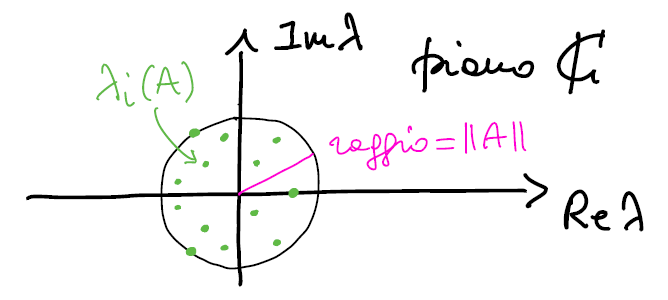
\includegraphics[scale=0.5]{lez19_img2.png}    
\end{center}
%PAGINA 32 \\%silvia

\begin{proof}[\unskip\nopunct]
\uline{Dimostrazione:}\\
Se $\lambda \in \mathbb{C}$ è autovalore di $A$ (ricordiamo ancora che gli autovalori di una matrice sono in generale complessi; se la matrice è reale vanno a coppie di complessi coniugati perché $det(\lambda I-A)$ ha coefficienti reali), per definizione $\exists \, x \ne 0$ autovettore tale che
\[Ax = \lambda x \quad (\text{cioè } (\lambda I-A)x = 0)\]
Usando la norma vettoriale che induce $\norma{A}$
\[\norma{\lambda x} \overset{(*)}{=} \abs{\lambda}\norma{x} = \norma{Ax} \le \norma{A}\norma{x}\]
[$(*)\, 2^{\circ}$ proprietà di una norma, vale anche per $\lambda \in \mathbb{C}$] \\
e dividendo per $\norma{x}$
\[\abs{\lambda} \le \norma{A}\]\\
\end{proof}
%PAGINA 33 \\ %Andrea

\subsection{TEOREMA (sull'invertibilità di $I-A$ per $\norma{A}<1$)}
\begin{center}
    \fbox{\begin{minipage}[t]{16cm}%
Sia $A \in \mathbb{R}^{n_x n}$ tale che $\norma{A}<1$, dove $\norma{A}$ è una qualsiasi norma matriciale indotta.\\
Allora $I-A$ è invertibile e vale la stima:
\begin{equation*}
    \norma{(I-A)^{-1}}\leq \frac{1}{1-\norma{A}}
\end{equation*}
\end{minipage}}
\end{center}
\begin{proof}[\unskip\nopunct]
\uline{Dimostrazione}\\
Innanzitutto osserviamo che gli autovalori di $I-A$, diciamoli $\mu_i$ tali che $det(\mu_iI-A)=0$,
%PAGINA 34\\%Andrea
sono $ \mu_i = 1 - \lambda_i (A)$, $1 \leq i \leq n$.\\
Infatti se $ A\ x = \lambda_i\ x$ con $x \neq 0$ allora:
\begin{equation*}
    (I-A)x = x-A x = x - \lambda_i x = (1- \lambda_i) x
\end{equation*}
cioè $x\neq 0$ è autovettore di $I-A$ relativo all'autovalore $1-\lambda_i$(cioè, gli autovalori di $I-A$ sono $\mu_i=\lambda_i(I-A)=1-\lambda_i(A)$ , $1\leq i \leq n$ mentre gli autovettori sono gli stessi).\\
Ma dal teorema di localizzazione sappiamo che $|\lambda_i(A)|\leq \norma{ A }< 1$ (perché $\norma{ A }$ è una norma indotta) quindi:
\begin{equation*}
    | \lambda_i(I-A) | = | 1-\lambda_i(A) | \geq \big | 1-|\lambda_i(A)| \big | = 1 - | \lambda_i(A) | > 0
\end{equation*}
%PAGINA 35\\%Andrea
cioè gli autovalori di $1-A$ sono tutti non nulli. \\
Di conseguenza $det(1-A)\neq 0$ ( perché il determinante di una matrice è il prodotto dei suoi autovalori) cioè $I-A$ è invertibile.\\
Chiamando $S = (I-A)^{-1}$ l'inversa di $I-A$, si ha $S(I-A) = I$. \\ Ma allora, visto che $\norma{I} = 1$ (perché $\norma{I} = \underset{x \neq 0}{sup}\norma{Ix}/\norma{x} =\underset{x \neq 0}{sup}\norma{x}/\norma{x} = 1 $, dove $\norma{x}$ è la norma vettoriale corrispondente)
\begin{equation*}
\begin{split}
1 =  \norma{I} = \norma{S(I-A)} = \norma{S-SA} \\ 
    \geq \Big | \norma{S} - \norma{SA} \Big | = \norma{S} - \norma{SA} \\
    \geq \norma{S} - \norma{S} \norma{A} = \norma{S} (1-\norma{A})
\end{split}
\end{equation*}
%PAGINA 36\\%Andrea
\begin{equation*}
    \text{perché} \  \norma{SA} \leq \norma{S} \norma{A} < \norma{S}\ \text{ visto che} \  \norma{A} < 1\\
\end{equation*}
Quindi possiamo scrivere
\begin{equation*}
    \norma{S} = \norma{(I-A)^{-1}} \leq \frac{1}{1-\norma{A}}
\end{equation*}
\end{proof}

Nella prossima lezione usando le norme vettoriali e matriciali studieremo la ``risposta" di un sistema lineare $n \times n$ non singolare agli errori sui dati, il cosiddetto problema del ``condizionamento".\\
\end{document}